\chapter{Approach}

In this section after describing the general convolutional architecture in spiking neural network, we discuss two different approaches to build convolutional deep belief networks.

The first one is the most classical one, where a offline/ in discrete time trained DBN is transferred to spiking neural networks.
The second approach trains the RBMs event based with STDP directly as spiking neural networks. 

\section{Convolutional architecture in spiking neural network}

We implement a convolutional layer with receptive fields and shared weights between two neuron populations. 
Each population has a similar 3 dimensional topology as in "normal" CNNs with the number of neurons given by $\# \text{neurons} = \text{channels} \times \text{height} \times \text{width}$.

Groups of neurons in the bottom layer in close vicinity, a so-called receptive fields, are each connected with synapses to a top layer neuron.
These receptive fields have the same size $n$ and shape and shared the same synaptic weights (given the top layer neurons belong to the same feature map).
The receptive fields are overlapping by $n-s$ neurons, where $s$ is the stride, and the output neurons have the same topology as their input regions. 
Recent state-of-the-art systems have mostly reached the common consensus, of choosing a stride of $s=1$, which we have adapted throughout this work.

The receptive fields cover partial regions of the input data, where the synaptic weights from the bottom layer neurons to the top layer neuron can the be seen as a convolution over the partial input data.
Since the weight of receptive field can be shared, the neural activity in the top layer can be seen as a convolution over the input data with a filter of the size of the receptive fields.
In this case the top layer activation of receptive fields with the same weights can also be called a feature map.

\begin{figure}
	\centering
	\begin{subfigure}[t]{.5\textwidth}
  		\centering
  		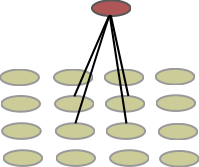
\includegraphics[width=.8\linewidth]{imgs/recpt_field1.png}
  		\caption{A subfigure}
  		\label{fig:sub1}
	\end{subfigure}%
	\begin{subfigure}[t]{.5\textwidth}
  		\centering
  		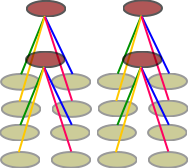
\includegraphics[width=.8\linewidth]{imgs/recpt_field2.png}
  		\caption{A subfigure}
  		\label{fig:sub2}
	\end{subfigure}
\end{figure}


By using more neurons with different set of shared weights over the same receptive fields, more feature maps can be implemented.     

\section{Conversion}

The conversion approach can be roughly described in two steps:
\begin{enumerate}
\item Train the RBMs to build up an DBN.
\item Convert the DBN to the spiking neural network.
\end{enumerate}


\subsection{Conv DBNs}

To train a convolutional DBNs we proceed similar to Hinton and Lee.

At first the convolutional RBMs are greedily trained with CD, as described in section 2.x, on images batches of batch-size $b$ for a certain number of iterations over the whole dataset, in this context referred to as epochs.
After a RBM is trained, we convert the dataset by sampling of the hidden layer of the RBM (one sampling/forward-pass step), into a new dataset:
\[
x' = \sigma(W * x) > rnd,
\]
where $rnd$ is a random number between $0$ and $1$.

On this converted dataset the next convolutional RBM is trained similar to the previous one.

Evaluating feature qualities is still an active top of research.
To get a measurement of our feature quality we use labeled data and train a classifier on top of the extracted features.
To stay in a biological plausible domain, we train a fully connected RBM on the top level features as well as the label of the data samples, to associate the features with the correct labels.
Out approach is similar to the approach of Hinton.

\begin{figure}
	\centering
    	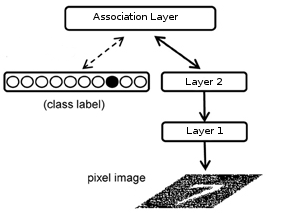
\includegraphics[width=0.4\textwidth]{imgs/dbn_mnist.png} 
    \caption{A figure.}
	\label{fig:test}
\end{figure}

To evaluate the final performance, we input a data sample without a label into the DBN and let the top layer sample a label prediction by performing Gibbs sampling steps.


\subsection{Conversion}

For the conversion we have three different variations

\begin{figure}
	\centering
	\begin{subfigure}[t]{.5\textwidth}
  		\centering
  		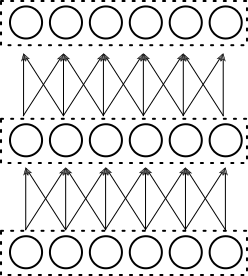
\includegraphics[width=.6\linewidth]{imgs/convert_cnn.png}
  		\caption{A subfigure}
  		\label{fig:sub1}
	\end{subfigure}%
	\begin{subfigure}[t]{.5\textwidth}
  		\centering
  		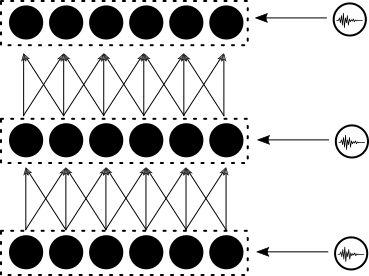
\includegraphics[width=.8\linewidth]{imgs/convert_dbn.png}
  		\caption{A subfigure}
  		\label{fig:sub2}
	\end{subfigure}
\end{figure}


\paragraph{Conversion as CNN} 

One way to convert the DBN to the spiking domain, is by interpreting it as a pretrained CNN with purely forward connections (we do not perform any commonly used gradient descent fine tuning to get comparable results with only CD trained models, but fine tuning could further improve the performance).

For the conversion, we proceed similar to Cao and Diehl.
They use avg pooling and ReLU functions, to get a similar architecture as SNNs.
In contrast, we don't use any pooling, since for RBM there is no simple way to integrate avg pooling (used by Cao and Diehl in their trained CNNs), and for spiking CNNs there is no simple way to integrate probabilistic max pooling, which is currently probably the only training integrated pooling thought of for RBMs.
We also use the sigmoid function, since RBMs are commonly trained with sigmoid activations (even so some approaches proposed ReLU for RBMs as well (see Hinton)) and the input-rate output-rate transfer function of rate based LIF neurons with a refractory period matches the sigmoid function more closely.

The DBN layers are replaced by a LIF neuron population layers with an identical architecture. 
The connections are replaced by (directed) synapses, with the weights of the DBN synapses scaled with a constant factor, to get similar activations.
 

\paragraph{Conversion with conductance-based LIF}

Another way to convert the DBN to the spiking domain, is by interpreting it as a directed graphical model, a sigmoid belief network, and perform ancestral sampling.

This approach is heavily based on the synaptic sampling theory, i.e. it uses spiking neurons to perform sampling.

The sampling can be either performed LIF neurons as described in 3.2.

For the COBA neurons, we choose a biological plausible neuron model (see parameters in table). 
The high conductance and increased mean potential (gaussian distributed) and thus a firing probabilty of .5, is achieved by using high frequency Poisson generated (inhibitory and exhibitory) spikes to bring the neuron to a high conductance state (HCS). 

This neuron model has an input-current/spikes to firing frequency mapping/ transfer function which approixmates a sigmoid function.


The PSP are chosen to have an alpha shape in stead of rectangular PSP, which as described in 3.2 may introduce some discrepancies when performing sampling in comparison to Gibbs sampling.

\begin{figure}
	\centering
	\begin{subfigure}[t]{.5\textwidth}
  		\centering
  		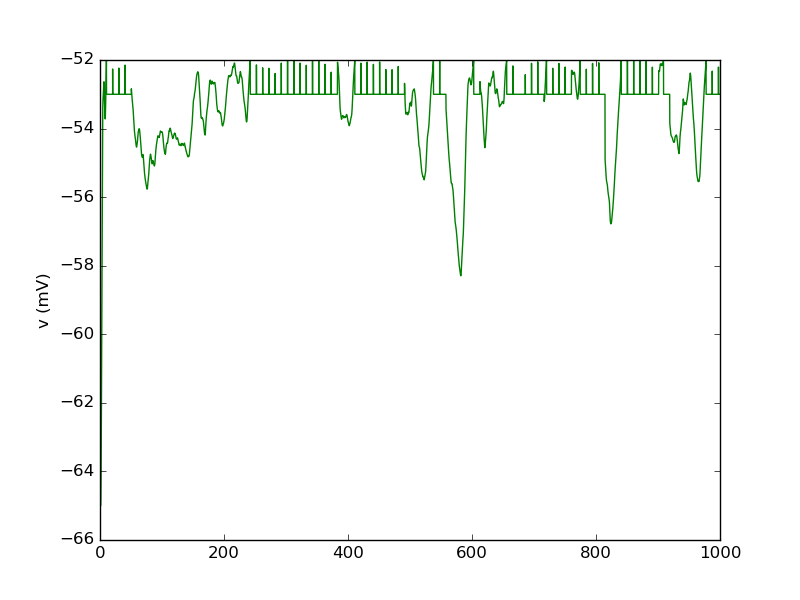
\includegraphics[width=.8\linewidth]{imgs/coba_lif_act.png}
  		\caption{A subfigure}
  		\label{fig:sub1}
	\end{subfigure}%
	\begin{subfigure}[t]{.5\textwidth}
  		\centering
  		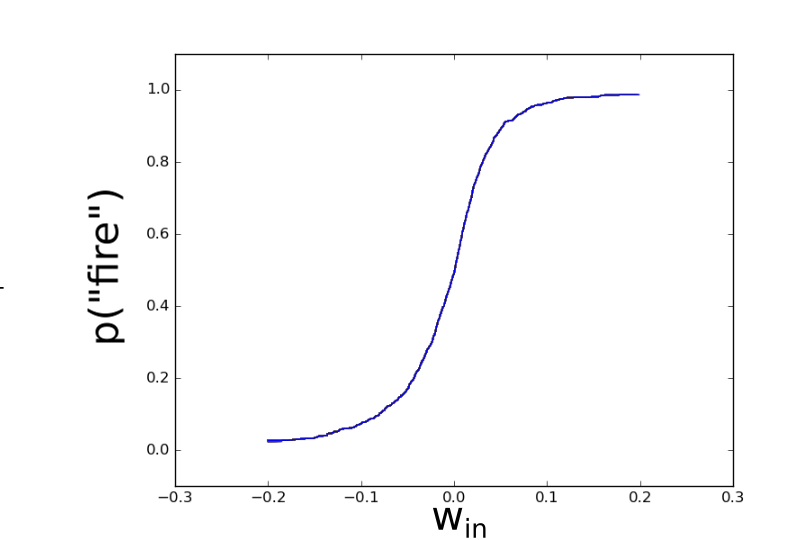
\includegraphics[width=.8\linewidth]{imgs/coba_lif_sigmoid.png}
  		\caption{A subfigure}
  		\label{fig:sub2}
	\end{subfigure}
	\begin{subfigure}[t]{.5\textwidth}
  		\centering
  		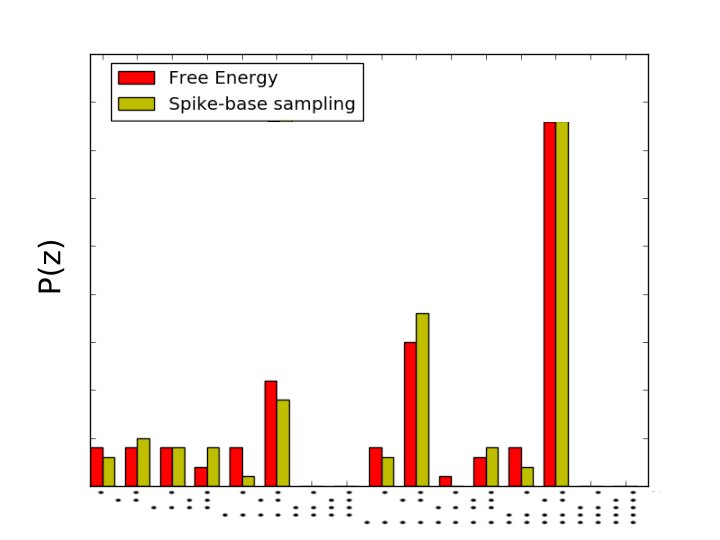
\includegraphics[width=.8\linewidth]{imgs/coba_lif_bm2.png}
  		\caption{A subfigure}
  		\label{fig:sub2}
	\end{subfigure}
\end{figure}
  
The DBN is converted by simply converting each layer to a layer of COBA LIFs with poisson noise, and the connections are transformed to synapses with the weights scaled to achieve a action function similar to the sigmoid function.

Consequently the DBN simply performs ancestral sampling with the data sample as evidences and the label as inferred state.   


\paragraph{Conversion with current-based LIF}

To reduce the computational expenses of the COBA models, they can be replaced by less computational complex CUBA models.

Their model parameters as chose to simulate a HCS state.

Therefore the membrane time constant as well as the membrane conductance are reduced and a static input current is inserted.  

By adding high frequency poisson noise, a sigmoid shaped input-rate output-rate transfer function is achieved.

\begin{figure}
	\centering
	\begin{subfigure}[t]{.5\textwidth}
  		\centering
  		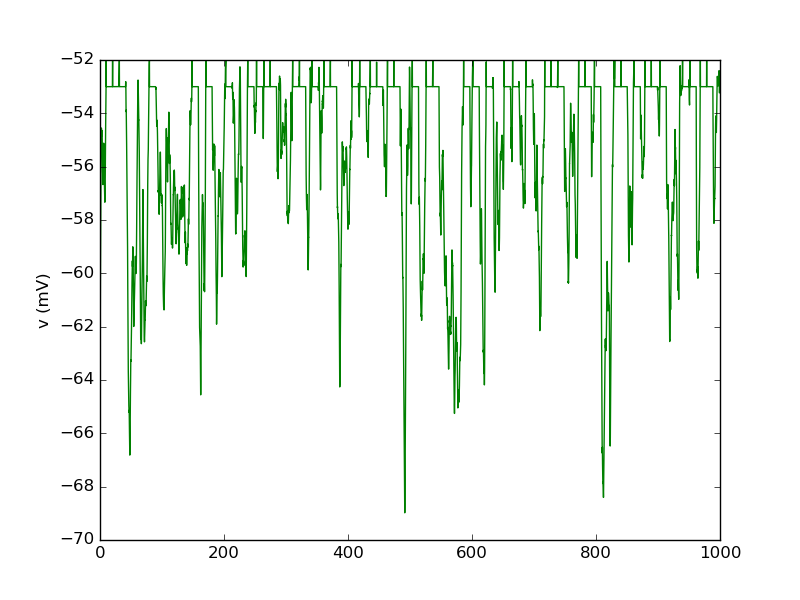
\includegraphics[width=.8\linewidth]{imgs/cuba_lif_act.png}
  		\caption{A subfigure}
  		\label{fig:sub1}
	\end{subfigure}%
	\begin{subfigure}[t]{.5\textwidth}
  		\centering
  		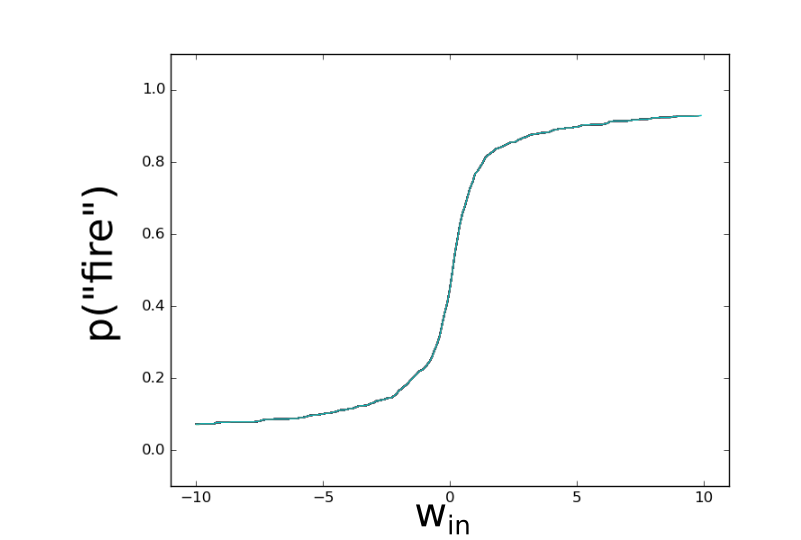
\includegraphics[width=.8\linewidth]{imgs/cuba_lif_sigmoid.png}
  		\caption{A subfigure}
  		\label{fig:sub2}
	\end{subfigure}
	\begin{subfigure}[t]{.5\textwidth}
  		\centering
  		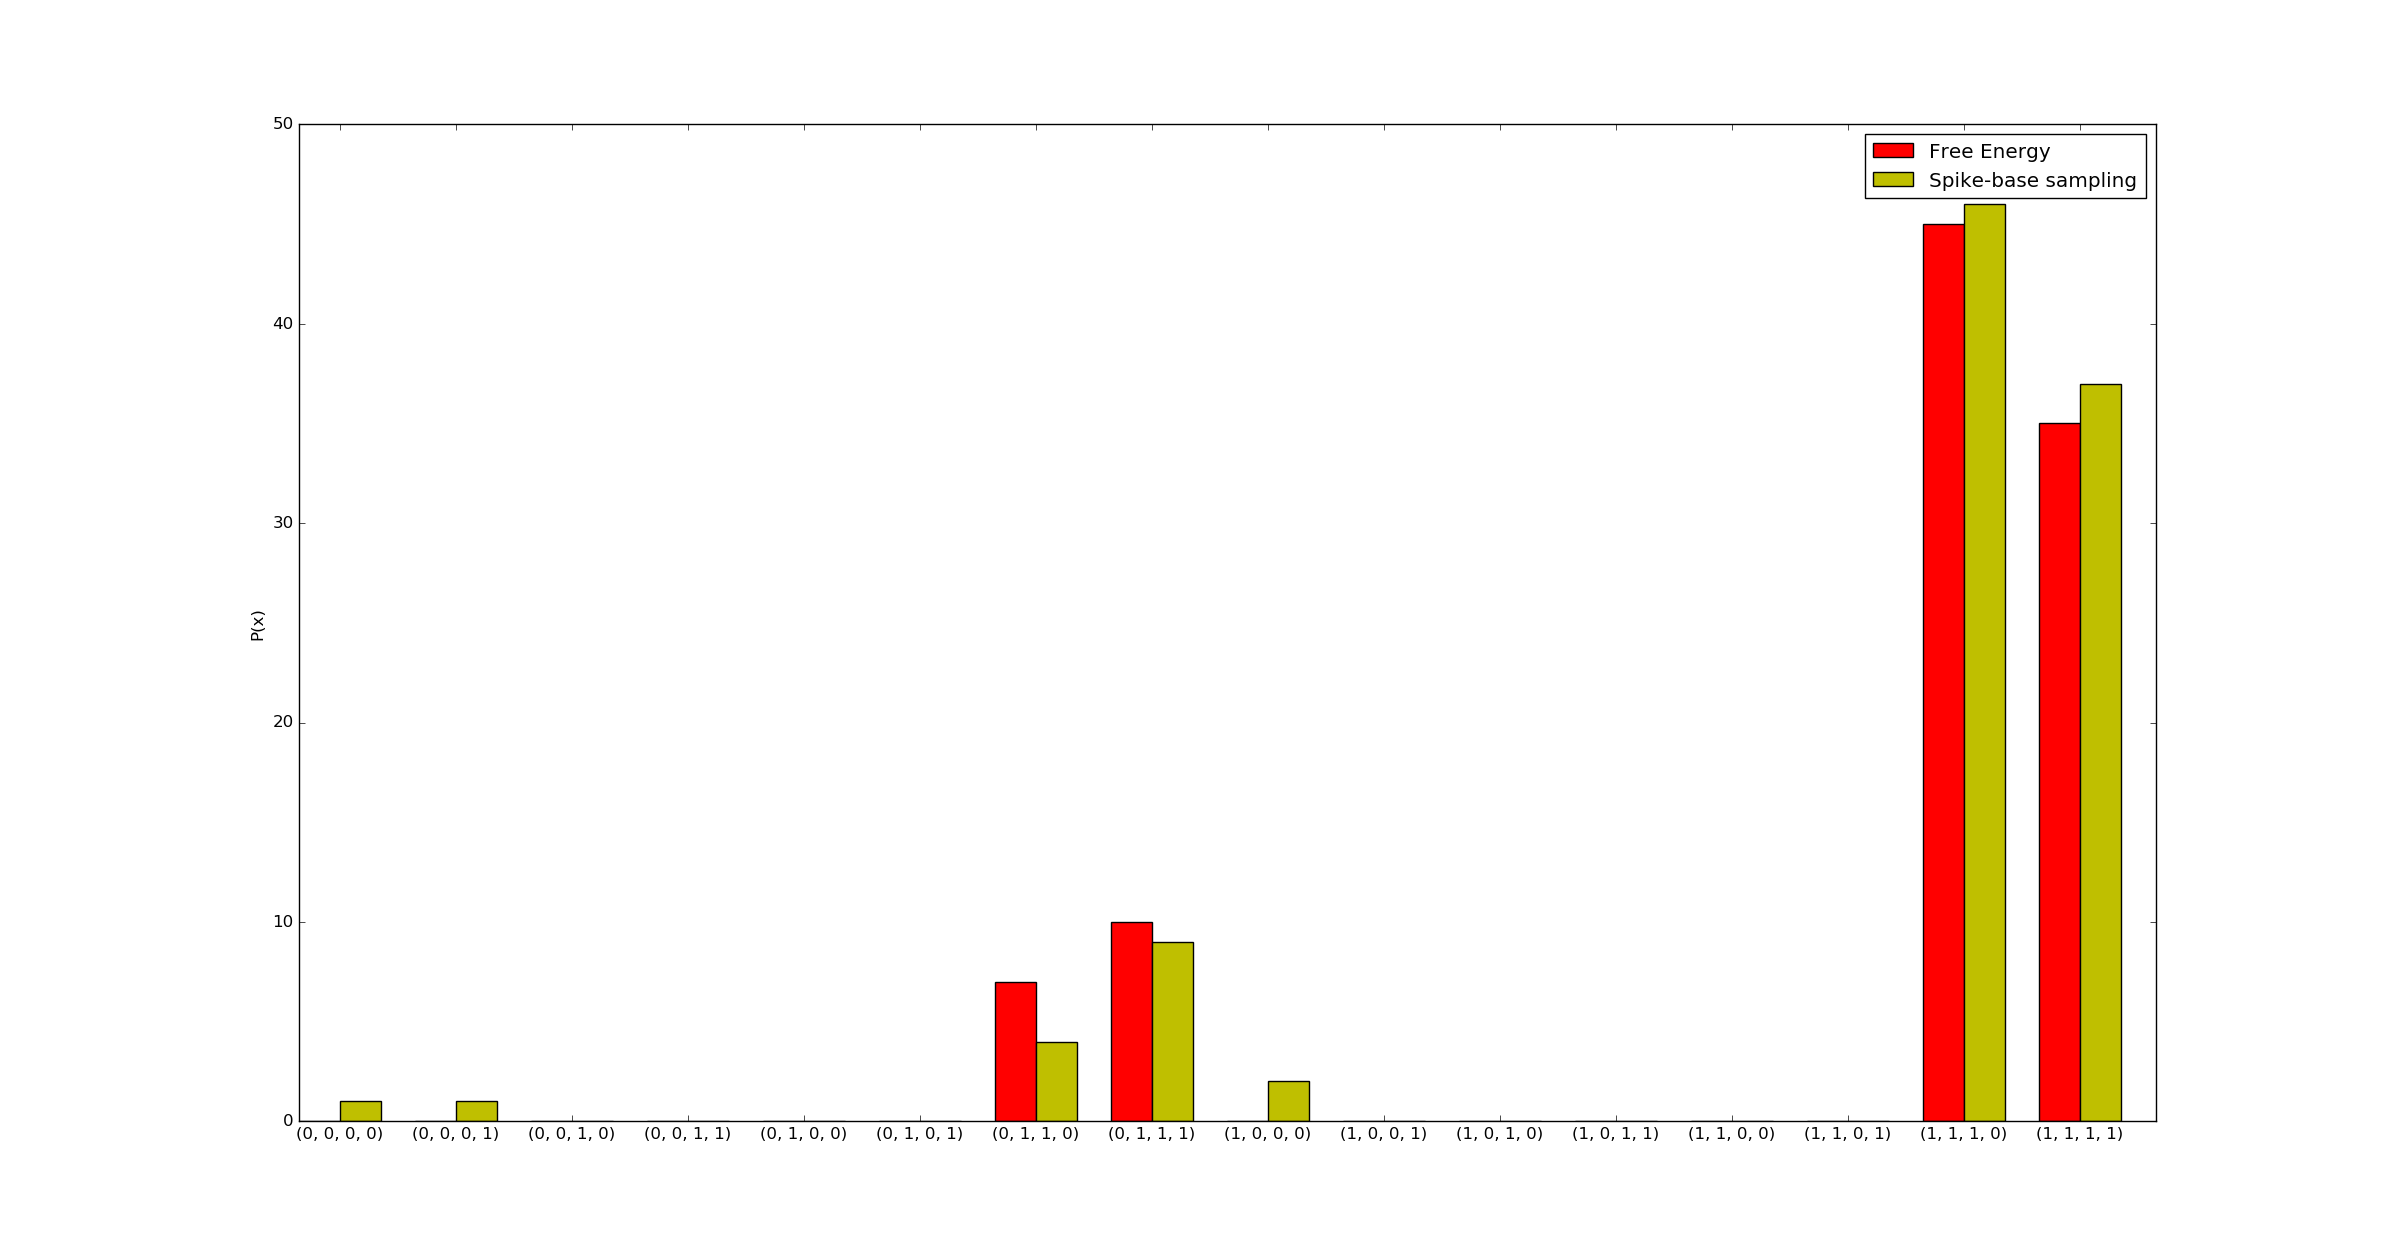
\includegraphics[width=.8\linewidth]{imgs/cuba_lif_bm.png}
  		\caption{A subfigure}
  		\label{fig:sub2}
	\end{subfigure}
\end{figure}
The DBN conversion is similar to the COBA case, where the COBA neurons are now replaced by the adapted CUBA LIFs.

\section{eCD}

Another approach tries to learn the convolutional spiking DBN with an STDP based learning rule. 

The main idea of the learning rule is adapted from Neftci.
We also use a LIF neuron model.
A similar STDP rule to the one described in 3.2 is used, but we extended the model with a learning rate. 
This rule can be reformulated as an iterative rule as follows:
\begin{itemize}
\item The visible unit $v$ spikes: 
\[
\begin{split}
A_v = A_v \exp(\frac{\Delta t}{\tau}) + a_{\delta} ,\\
A_h = A_h \exp(\frac{\Delta t}{\tau}) ,\\
\delta w = g(t) \mu A_v  ,\\
\end{split}
\]
\item The visible unit $h$ spikes: 
\[
\begin{split}
A_h = A_h \exp(\frac{\Delta t}{\tau}) + a_{\delta} ,\\
A_v = A_v \exp(\frac{\Delta t}{\tau}) ,\\
\delta w = g(t) \mu A_h  ,\\
\end{split}
\]
\end{itemize}
where $g(t)$ is the STDP status flag, $\Delta t$ is the time difference to the last previous spike, and $a_{delta}$ represents the input of a Dirac-shaped spike train.


The original division into four training phases poses similarites to pCD since the activity of the hidden layer of the previous step is used as starting state for the next step, we extent the model by a 5th phase between the two data samples, where the model is "flushed" thus enabling normal CD:

\begin{enumerate}
\item The data signal is applied and the system is allowed to model the data distribution ($g(t)=0$)
\item Positive STDP is used to get $v_i h_j$-data (with stdp) and is added to the weights (postive phase $g(t)=1$)
\item The data signal is remove and the system is allowed to model the model distribution ($g(t)=0$)
\item Negative STDP is used to get $v_i h_j$-model (with stdp) and is substracted from the synaptic weights (negative phase $g(t)=-1$).
\item The neural activity is "flushed" by inserting a strong negative current into the visible and hidden layer, to learning is performed ($g(t)=0$).
\end{enumerate}

\begin{figure}
	\centering
    	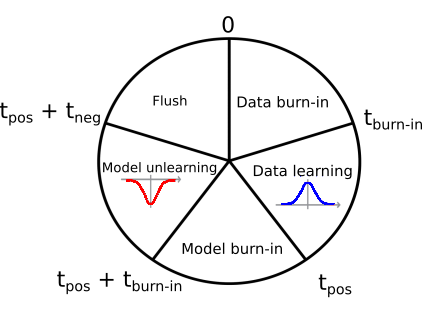
\includegraphics[width=0.4\textwidth]{imgs/eCD_5phases.png} 
    \caption{A figure.}
	\label{fig:test}
\end{figure}

$STDP CURVE$

\subsection{Convolution}

We implement convolution with local receptive field and sharing weights between neuron through weight synchronization.
Since each weight has their local STDP based update rule (eCD), we have to find a way to synchronize/share weights between all neurons in a layer.
To keep the weights in neuron in a layer the same, we perform a weight synchronization step at discrete time steps, since updating all weights after a single update did not show any promising results.
Thus the synchronization at a time step for weight shared weights $w_i$ , $w_j$ can be described by the following rule:  
\[
\begin{split}
w_i(t) = w_{shared}(t-1) + \delta w_i, \\ 
w_j(t) = w_{shared}(t-1) + \delta w_j 
\end{split}
\]
which gives the new shared weight
\[
\begin{split}
w_{shared}(t) = \frac{1}{2} (w_i(t) + w_j(t) ) = \frac{1}{2} (w_{shared}(t-1) + \delta w_i + w_{shared}(t-1) + \delta w_j) = \\ w_{shared}(t-1) + \frac{1}{2} (\delta w_i + \delta w_j).
\end{split}
\]

This results in a update rule similar to the convolutional RBM update rule 3.x.
Thus we can simply take the mean of the weight changes and apply it to all the weights, which is equivalent to just taking the average of the new individual weights. 

\paragraph{Lateral inhibition}
In addition we introduce fixed negative connections between neuron in the top/ hidden layers (biological plausible --> more sparse King).
This removes one advantage of RBMs since the hidden layers are no longer independed, which makes it harder to sample from the true distributions, but since the network continuously performs sampling steps, the approximation is is sufficient, if the weights are not to strong and prevent a change to a different mode.

\begin{figure}
	\centering
    	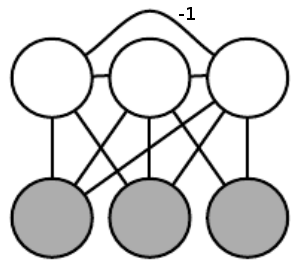
\includegraphics[width=0.4\textwidth]{imgs/lateral_inhib.png} 
    \caption{A figure.}
	\label{fig:test}
\end{figure}


By connecting neurons to neurons on a similar positions in other feature maps, appears to make the features more discriminative and less correlated.
Also this poses some similarities to adding a negative structured bias to the hidden units, which has shown to result in better features (see Norouzi M).

An intuitive interpretation, is that if one feature reacts to a certain input it will be highly active and prevent the others from being active as well and thus prevent them from learning the same.  

\subsection{Spiking DBNs}

To build up a spiking DBN we train the convolutional BMs layer-wise and forward the input of the previous layer to the next layer.

To be exact the spiking DBN is a mixture between a DBN and a DBM, since the single BMs are still bidirectional connected and only the hidden layer is forwarded in a directed manner.
Converting a RBM to a directed BN did not show any good results, since the activation of the hidden unit turned out to be important for generating a good estimate of the data distribution. 

$IMAGE$

Due to some top-down influences, when stacking a new BM on the trained BM, the hidden distribution gets distorted and unfit input for the new BM to be trained on. 
To solve this in our case we simply use forward connections from the hidden activations to the input layer of a new two layered BM. 
An approach similar to Salakhutdinovs DBMs with doubling the weights and composing the models in the end may sound promising and could be tried as well.

\begin{figure}
	\centering
    	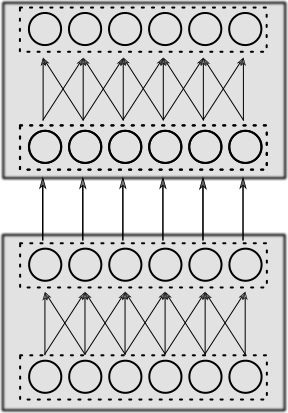
\includegraphics[width=0.4\textwidth]{imgs/spike_dbn.png} 
    \caption{A figure.}
	\label{fig:test}
\end{figure}

